\section{Structure-Aware Incremental Maintenance}
\label{sec: maintenance}



\subsection{Structural Classification of Edge Updates}




As the graph dynamically inserts or deletes vertices or edges, this may affect GIR layers in different ways.
However, we observe that many updates actually leave the structural connectivity entirely unchanged. For example, an edge inserted within a WCC would not alter that WCC at all. 
% For example, an edge inserted within a WCC would not alter that WCC at all.

To leverage this opportunity, we design a \textit{structure-aware incremental maintenance method to identify exactly which regions are affected and repair only the minimum necessary ones}.
% To address it, we design two complementary strategies, i.e., \textit{Scope-Prune-Update (SPU) for single update}, and \textit{Filter-Merge-Update (FMU) for batch update}.
Particularly, GIR's three-layer hierarchy transforms the maintenance problem.
Instead of treating every edge change as a potential graph-wide event, \textit{we classify each update into one of five distinct cases using only pre-maintained metadata}.
Each case identifies exactly which layers are affected and confines the repair to the smallest possible region.
We call this strategy \textit{Scope-Prune-Update (SPU)} for single-edge updates and extend it to \textit{Filter-Merge-Update (FMU)} for batches.

We primarily focus on \textit{single edge update} (insertion or deletion), as vertex insertions without edges do not affect connectivity and vertex deletions reduce to bulk edge deletions.
The central challenge is determining which GIR layers each operation affects.
Because GIR stores component labels, SCC membership, DAG ranks, and articulation point metadata for every vertex, it resolves this question through a metadata lookup, not a graph traversal.
This classification is only possible as GIR maintains all three structural layers simultaneously.
% No system that lacks these layers can make such a distinction.
% \YJ{working on.}

Every edge update ($s\rightarrow t$) falls into one of five cases shown in Figure~\ref{fig:scope-update}.
Particularly, \circled{c1}~$s$ and $t$ reside in \emph{different WCCs} (insertion);
\circled{c2}~$s$ and $t$ reside in the \emph{same WCC but different SCCs} (insertion);
\circled{c3}~$s$ and $t$ reside in the \emph{same SCC but different BiCCs} (insertion);
\circled{c4}~$s$ and $t$ reside in the \emph{same BiCC} (insertion);
\circled{c5}~edge \emph{deletion}, whose scope depends on bridge status.
In addition, Table~\ref{tab:updates} summarizes the scope rules and time complexity.
For each case, we identify which GIR layers are affected (\textit{scope}), how GIR restricts computation to the smallest subgraph (\textit{prune}), and what structural repair GIR performs (\textit{update}). 
% Below, we will discuss the details for each case.

\begin{figure}[t]
    \centering
    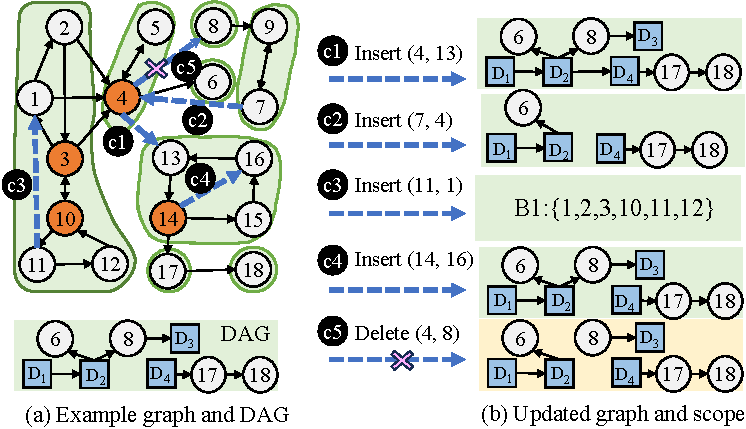
\includegraphics[width=1\linewidth]{figures/update_scope-crop.pdf}
    \caption{Five cases (\circled{c1}-\circled{c5}) for a single edge update.
    % Cases \circled{c1}-\circled{c4} are about insertions,
    % % classified by the structural relationship between the two endpoints; 
    % while \circled{c5} is about deletion.
    % classified by whether the removed edge is a bridge and at which GIR layer.
    Affected DAG nodes are highlighted in blue, and green shade indicates a WCC.}
    % \YJ{X on the deletion edge.}}
    \label{fig:scope-update}
\end{figure}


\begin{table}[t]
    \centering
    % \footnotesize
    \setlength{\tabcolsep}{3pt}
    % \renewcommand{\arraystretch}{1.1}
    \caption{Scope rules and SPU time complexity per case.
    $|V_{\mathrm{a}}|$ and $|E_{\mathrm{a}}|$ denote the number of vertices and edges in the affected region;
    $\Delta r$ denotes the rank interval for Case~2.}
    \begin{tabular}{c l c l l}
    \toprule
    \textbf{Case} & \textbf{Endpoint relation} & \textbf{Op} & \textbf{Layers} & \textbf{Complexity} \\
    \midrule
    1  & Different WCCs                         & Ins & WCC             & $\mathcal{O}(1)$ \\
    \multirow{2}{*}{2}
       & \multirow{2}{*}{Same WCC, diff.\ SCCs} & \multirow{2}{*}{Ins}
                                                & SCC (no cycle)  & $\mathcal{O}(1)$ \\
       &                                        &     & SCC+BiCC        & $\mathcal{O}(\Delta r$+$|V_{\mathrm{a}}|$+$|E_{\mathrm{a}}|$) \\
    3  & Same SCC, diff.\ BiCCs                 & Ins & BiCC            & $\mathcal{O}(|V_{\mathrm{a}}|+|E_{\mathrm{a}}|)$ \\
    4  & Same BiCC (no-op)                      & Ins & BiCC             & $\mathcal{O}(1)$ \\
    \midrule
    5a & Non-bridge                             & Del & BiCC            & $\mathcal{O}(|V_{\mathrm{a}}|+|E_{\mathrm{a}}|)$ \\
    5b & Bridge within SCC                      & Del & SCC+BiCC        & $\mathcal{O}(|V_{\mathrm{a}}|+|E_{\mathrm{a}}|)$ \\
    5c & Bridge in DAG                          & Del & WCC+BiCC        & $\mathcal{O}(|V_{\mathrm{a}}|+|E_{\mathrm{a}}|)$ \\
    \bottomrule 
    \end{tabular}
    \label{tab:updates}
\end{table}


\textbf{Case 1 (Insertion): $s$ and $t$ reside in different WCCs.}
The inserted edge connects two previously disconnected regions.
No directed cycle can form across WCC boundaries, and thus no biconnected structure inside either component changes.

\textit{Scope.} GIR identifies WCC layer as the only affected layer.

\textit{Prune and Update.} GIR merges the two components in $O(1)$ time via a
union-find root-pointer update~\cite{tarjan1975efficiency}: only the root label
of the smaller component is redirected to the root of the larger one, with no
SCC or BC tree traversal.
Full path compression is applied lazily during subsequent label lookups, keeping
amortized per-operation cost at $O(\alpha(n))$.
% \CQ{The time complexity is $\mathcal{O}(1)$, as the merge requires only a single WCC label update with no SCC or BiCC traversal.}


\textit{Example.}
Inserting an edge $(4,\,13)$ (\circled{c1} in Figure~\ref{fig:scope-update})
% (\circled{c1}) 
bridges $\text{WCC}_1 = \{1, ..., 12\}$ and $\text{WCC}_2 = \{13, ..., 18\}$.
Thus, GIR connects the two condensation DAGs into one.





\textbf{Case 2 (Insertion): $s$ and $t$ are in the same WCC but different SCCs.}
The inserted edge $s \to t$ introduces a new edge between two SCC supernodes in the condensation DAG.
The critical question is \textit{whether this edge creates a directed cycle, which would cause two or more SCCs to merge}.

\textit{Scope.} To answer this without traversing the entire DAG, we design a rank-based method. 
That is, we assign each SCC a {rank}, which is a compact topological index maintained incrementally alongside the DAG.
If $\mathrm{rank}(\mathrm{SCC}(s)) \le \mathrm{rank}(\mathrm{SCC}(t))$, the edge either follows the existing DAG order or connects two SCCs at the same rank with no directed path between them.
Neither will form a cycle, and the scope is limited to inserting a new DAG edge with no SCC-level structural change.
If $\mathrm{rank}(\mathrm{SCC}(s)) > \mathrm{rank}(\mathrm{SCC}(t))$, the edge goes against the DAG order and may introduce a cycle.
The scope then expands to the SCC and BiCC layers.

\textit{Prune.} 
% As illustrated in Figure~\ref{fig:rank-prune},
GIR restricts cycle detection to the rank interval $[\mathrm{rank}(\mathrm{SCC}(t)),\,\mathrm{rank}(\mathrm{SCC}(s))]$ in the  DAG.
This avoids a global DAG search.

\textit{Update.} If a cycle is detected within this interval, it merges all SCCs on this cycle, updates the condensation DAG locally, and reconstructs the BC trees of the affected SCCs. The time complexity is $\mathcal{O}(\Delta r + |V_{\mathrm{a}}| + |E_{\mathrm{a}}|)$, where $|V_{\mathrm{a}}|$ and $|E_{\mathrm{a}}|$ denote vertex and edge count of  the affected region, and $\Delta r$ denotes the rank interval.
If no cycle forms, the cost is $\mathcal{O}(1)$. 

% When a cycle is detected, the rank-interval search costs $\mathcal{O}(\Delta r)$ and the SCC merge plus BC tree reconstruction costs $\mathcal{O}(|V_{\mathrm{aff}}| + |E_{\mathrm{aff}}|)$, giving a total of $\mathcal{O}(\Delta r + |V_{\mathrm{aff}}| + |E_{\mathrm{aff}}|)$.

\textit{Example.}
As shown in Figure~\ref{fig:rank-prune}, inserting edge $(7,\,4)$ (\circled{c2}) has $\mathrm{rank}(D_3) > \mathrm{rank}(D_2)$. As $D_2 \to D_3$ is in the original DAG, the edge goes against the DAG order and triggers cycle detection over $[\mathrm{rank}(D_2),\,\mathrm{rank}(D_3)]$.
A cycle is found, and $D_2$ and $D_3$ will be merged.
The BC tree of the combined SCC will be updated, as shown in Figure~\ref{fig:scope-update} (\circled{c2}).
In contrast, inserting $(2,\,8)$ satisfies $\mathrm{rank}(\mathrm{SCC}(2)) \le \mathrm{rank}(\mathrm{SCC}(8))$, thus no cycle can form and only a new DAG edge is added.



\textbf{Case 3 (Insertion): $s$ and $t$ are in the same SCC but different BiCCs.}
Both endpoints lie within the same SCC, so no WCC or SCC needs to be changed.

\textit{Scope.} GIR confines the scope to the BiCC layer. Specifically, only the two BiCC blocks containing $s$ and $t$ are potentially affected.

\textit{Prune and Update.} The new edge may merge the two blocks into a single larger BiCC, eliminating one or more APs.
GIR updates the BC tree accordingly.
The time complexity is $\mathcal{O}(|V_{\mathrm{a}}| + |E_{\mathrm{a}}|)$, confined to the two affected BiCC blocks and the local BC tree repair.

\begin{figure}[t]
    \centering
    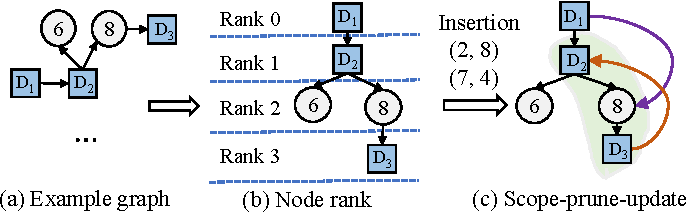
\includegraphics[width=1\linewidth]{figures/scope_update-crop.pdf}
    \caption{Rank-interval pruning for Case \circled{c2} (inter-SCC insertion). 
    Inserting edge (2, 8) will not affect SCC, while edge (7, 4) will merge multiple SCCs.
    % Each SCC is assigned a topological rank in the condensation DAG. When an inserted edge goes against the DAG order from $\mathrm{SCC}(s)$ to $\mathrm{SCC}(t)$, GIR restricts cycle detection to the rank interval $[\mathrm{rank}(\mathrm{SCC}(t)),\,\mathrm{rank}(\mathrm{SCC}(s))]$ (shaded region), avoiding a global DAG traversal.
    %\YJ{Make sure this figure matches with the example in Figure 5.} done it;s the same
    }
    \label{fig:rank-prune}
\end{figure}
\textit{Example.}
Inserting an edge $(11,\,1)$ (\circled{c3} in Figure~\ref{fig:scope-update}) will lead to the merge of two blocks. Particularly, 
vertex $11$ is in block $B_1 = \{10,\,11,\,12\}$ and vertex $1$ is in block $B_2 = \{1,\,2,\,3\}$, both within $D_1$.
Therefore, GIR merges the two blocks into $B_1 = \{1,\,2,\,3,\,10,\,11,\,12\}$.
% , as shown in Figure~\ref{fig:scope-update} (\circled{c3}).


\textbf{Case 4 (Insertion): $s$ and $t$ are in same BiCC.}
As both vertices already belong to the same BICC, adding an edge within an already 2-edge-connected subgraph will not create new APs, split any BiCC, or alter SCC or WCC structure.

\textit{Scope.} GIR identifies the update as a structural no operation for all layers.
The time complexity is $\mathcal{O}(1)$.
% and no maintenance is needed.
% \CQ{Since no structural change occurs, the time complexity is $\mathcal{O}(1)$.}


\textit{Example.}
Inserting an edge $(14,\,16)$ (\circled{c4} in Figure~\ref{fig:scope-update}) will not change the GIR as both vertices lie in the same block $D_4$.
% so the GIR remains unchanged (Figure~\ref{fig:scope-update}, \circled{c4}).

\textbf{Case 5 (Deletion):}
The scope of deleting an edge $(s,\,t)$
depends on whether the edge is a bridge, which is defined as the only edge between two blocks.
%\YJ{clearly explain what is an bridge.} 
For this case, GIR further decomposes it into three sub-cases.


\emph{Case 5a (non-bridge):}
If parallel edges or alternative undirected paths exist between $s$ and $t$, the deletion cannot change WCC, SCC, or higher-level connectivity.
GIR confines the scope to the BiCC layer, checks whether any articulation points have changed, and repairs the BC tree locally within the enclosing SCC.
% \CQ{
The time complexity is $\mathcal{O}(|V_{\mathrm{a}}| + |E_{\mathrm{a}}|)$, confined to the affected BiCC block within the enclosing SCC.
% }


% \emph{Case 5a (non-bridge):}
% If parallel edges or alternative undirected paths exist between $s$ and $t$, the deletion cannot change WCC, SCC, or higher-level connectivity.
% \textit{Scope.} GIR confines the scope to the BiCC layer: the removed edge may alter block boundaries or articulation structure within the enclosing SCC, but the change does not propagate upward.
% \textit{Update.} GIR checks whether any articulation points have changed and repairs the BC tree locally.

\emph{Case 5b (bridge within an SCC):}
% If the edge is the unique undirected path between its endpoints and both endpoints share the same SCC, the deletion may split that SCC.
% \textit{Scope.} GIR expands the scope to the SCC layer: it checks whether the directed SCC breaks apart.
% If so, GIR partitions the affected SCC, rebuilds the relevant fragment of the condensation DAG, and reconstructs the BC trees of the resulting components.
If the edge is a bridge and both endpoints share the same SCC, GIR expands the scope to the SCC layer.
It checks whether the directed SCC breaks apart and, if so, partitions the affected SCC, rebuilds the relevant fragment of the condensation DAG, and reconstructs the BC trees of the resulting components.
% \CQ{
The time complexity is $\mathcal{O}(|V_{\mathrm{a}}| + |E_{\mathrm{a}}|)$, covering the SCC partition check, condensation DAG fragment update, and BC tree reconstruction.

\emph{Case 5c (bridge in the condensation DAG):}
If the deleted edge is an inter-SCC edge and serves as the bridge connecting two regions of the WCC, its removal disconnects the WCC entirely.
In this situtation, both WCC and BiCC layers are affected. It will split the WCC into two independent components, partition the condensation DAG accordingly, and update the BC trees on each side to reflect the new component boundaries.
The time complexity is $\mathcal{O}(|V_{\mathrm{a}}| + |E_{\mathrm{a}}|)$, covering the WCC split, condensation DAG partition, and BC tree updates on both resulting components.

\textit{Example.} 
The edge $4 \to 8$ (\circled{c5} in Figure~\ref{fig:scope-update}) 
% Deleting bridge $(4,\,8)$ (\circled{c5}): edge $4 \to 8$ 
is the only edge between the $\{D_1, D_2\}$ side and the $\{6, 8, D_3\}$ side.
% of the graph.
Deleting it will split the WCC into two, which will lead to WCC relabeling and BC tree updating on each resulting component.
% \CQ{

% }



% \emph{Case 5c (bridge in the condensation DAG):}
% If the deleted edge is an inter-SCC arc and serves as the only undirected path connecting two regions of the WCC, its removal disconnects the WCC entirely.

% \textit{Scope.} GIR identifies both the WCC and BiCC layers as affected: it splits the WCC into two independent components, partitions the condensation DAG accordingly, and updates the BC trees on each side to reflect the new component boundaries.

% \textit{Example.}
% Deleting bridge $(4,\,8)$ (\circled{c5}): edge $4 \to 8$ is the only undirected path between the $\{D_1, D_2\}$ side and the $\{6, 8, D_3\}$ side of the graph.
% GIR splits the WCC into two components, as shown in Figure~\ref{fig:scope-update} (\circled{c5}), and performs WCC relabeling and BC tree updates on each resulting component.


% \textit{Example.}
% Deleting bridge $(4,\,8)$ (\circled{c5}): edge $4 \to 8$ is the only undirected path between the $\{D_1, D_2\}$ side and the $\{6, 8, D_3\}$ side of the graph.
% GIR splits the WCC into two components, as shown in Figure~\ref{fig:scope-update} (\circled{c5}), and performs WCC relabeling and BC tree updates on each resulting component.




%if 5 == all, all the edges are included, insertion and deletion are within those cases.

% Table~\ref{tab:updates} summarizes the scope rules and per-case time complexity.
% \CQ{Three cases cost $\mathcal{O}(1)$: Case~1 (WCC merge) requires only a label update; Case~2 without a cycle adds a single DAG edge; Case~4 is a structural no-op that touches no GIR layer.
% Case~2 with a cycle costs $\mathcal{O}(\Delta r + |V_{\mathrm{aff}}| + |E_{\mathrm{aff}}|)$, where $\Delta r$ bounds the rank-interval cycle search and $|V_{\mathrm{aff}}| + |E_{\mathrm{aff}}|$ covers the SCC merge and BC tree reconstruction within the identified interval.
% Cases~3, 5a, 5b, and 5c all cost $\mathcal{O}(|V_{\mathrm{aff}}| + |E_{\mathrm{aff}}|)$, where the affected region is always confined to the structurally identified subgraph: the two BiCC blocks for Case~3, the enclosing BiCC block for Case~5a, the affected SCC and its condensation DAG fragment for Case~5b, and both resulting WCC components with their BC trees for Case~5c.
% Crucially, $|V_{\mathrm{aff}}| + |E_{\mathrm{aff}}|$ is always a strict subgraph of $G$, so SPU never performs a full-graph traversal regardless of graph size.}

% \subsection{Region-Minimal Layered Repair}

% \subsection{Top-down Cascaded Repair}

% The five-case classification identifies \emph{which} layers are affected. 
% % tells GIR \emph{which} layers are affected.
% The follow-up challenge is to correctly apply them on the GIR.
% To achieve that, we design a top-down cascaded repair method 
% % reginon-minimal layered repair method 
% to confine and execute the repair to guarantee that no update touches more structure than logically necessary.

% The key design principle is \textbf{top-down cascaded repair}, i.e., GIR always repairs layers from coarsest to finest.
% It first stabilizes the WCC layer, then the SCC/DAG layer, then the BiCC/BC tree layer.
% Each layer's repair is confined to the region that the layer above it identifies as affected.
% This cascade ensures that lower-layer repairs never operate on stale higher-layer state.

% \textit{WCC-layer repair.}
% WCC repair is the simplest.
% For Case~1 insertions, GIR merges two WCCs with a single relabeling step.
% For Case~5c deletions, GIR splits a WCC by checking connectivity and assigning new component labels.
% Both operations are $O(1)$ or $O(|V_{\mathrm{WCC}}|)$ in the affected component.
% No other case triggers WCC repair.

% \textit{SCC/DAG-layer repair.}
% SCC repair is governed by cycle formation (insertion) or cycle breaking (deletion).
% For Case~2, the rank-interval pruning (Figure~\ref{fig:rank-prune}) bounds the cycle search to a small region of the condensation DAG.
% If GIR finds a cycle, it merges the involved SCCs and locally updates the DAG.
% For Case~5b, GIR checks whether the deleted bridge disconnects the directed SCC.
% If so, GIR partitions the SCC, updates the DAG fragment, and passes the resulting sub-SCCs to the BiCC layer for BC tree reconstruction.
% In both cases, GIR touches only the SCCs within the pruned interval, not the entire DAG.

% \textit{BiCC/BC tree repair.}
% BiCC repair runs only after the WCC and SCC layers have stabilized.
% For Case~3, GIR merges the two affected BiCC blocks and removes the eliminated articulation points from the BC tree.
% For Cases~5a and 5b, GIR checks whether the deletion creates new articulation points or splits existing blocks, and repairs the BC tree accordingly.
% Because the higher layers have already localized the affected SCC, BC tree repair is confined to a small subgraph.
% Within a large SCC, GIR can carry out multiple non-overlapping BiCC repairs in parallel.

% This layered discipline produces a strong guarantee, that the repair never performs more  than the structural change requires.

\subsection{Filter-Merge-Update for Batch Updates}

Applying the single edge update strategy (SPU) independently to each update in a batch is correct but inefficient.
% Two problems arise.
There are two problems.
\textit{(i)} Some updates cancel or are redundant. That is, if an edge is inserted and later deleted within the same batch, neither needs to be processed.
\textit{(ii)} Multiple updates may jointly affect the same structural region.
Processing them one at a time triggers repeated maintenance on the same region.

To address both problems, 
we design a filter-merge-update (FMU) strategy by preprocessing the batch before applying SPU logic. Specifically, it involves three stages.

\textit{(i) Filter} stage removes updates that does not require processing.
Particular, we identify two such types of updates.
The first is canceling pair. 
% \emph{Canceling pairs:} 
That is, if an edge is inserted and later deleted within the same batch (or vice versa), the two operations cancel and GIR discards both.
The second is structural no operations.
% \emph{Structural no-ops:} 
Particularly, based on the five-case classification
% each remaining update using the five-case rules
in Table~\ref{tab:updates}, we remove any Case~4 updates (i.e., $s$ and $t$ are in the same BiCC), as they will not affect any GIR layer.
% Particularly, GIR classifies each remaining update using the five-case rules in Table~\ref{tab:updates} and removes any Case~4 updates (i.e., $s$ and $t$ are in the same BiCC) immediately, since they cannot affect any GIR layer.
This filter step reduces both the number of updates and the total maintenance work.

\textit{(ii) Merge}
% After filtering, GIR 
will group the remaining updates by the structural region they may jointly affect.
We first group the updates whose endpoints share the same WCC.
Within each WCC group, we identify updates whose SCC endpoints have overlapping DAG rank intervals and merges them into a single SCC-level maintenance region.
Further, we group updates that touch the same local articulation structure at the BiCC level.
This grouping has two benefits.
First, it amortizes repeated maintenance. That is, the updates that would trigger repairs on the same region are handled together in a single pass.
Second, it identifies structurally independent groups, each of which becomes a natural unit for parallel execution.

\textit{(iii) Update.}
Finally, GIR applies the single edge update logic to each merged region rather than to individual edges.
A set of inserted edges may jointly create a cycle and merge several SCCs, even though none of the edges alone would trigger a merge.
GIR detects such structural transitions over the merged region and repairs the corresponding WCC, SCC, and BC tree structures in a coordinated way.
Once the batch is complete, GIR processes independent merged regions concurrently.
This makes FMU a parallel and amortized extension of SPU for high-throughput update streams.

% Together, SPU and FMU keep GIR structurally consistent under both fine-grained and high-throughput updates.





% % As the graph will dynamically insert or delete nodes or edges, this may affect GIR layers in different ways.
% % % edge insertion or deletion may affect GIR layers in different ways.
% % However, we observe that many updates actually leave the structural connectivity entirely unchanged. For example, an edge inserted within a WCC would not after that WCC at all. 
% % To leverage this opportunity, \textit{the key challenge is to identify exactly which layers are affected and repair only the minimum necessary region}.
% % To address it, we design two complementary strategies, i.e., \textit{Scope-Prune-Update (SPU) for single update}, and \textit{Filter-Merge-Update (FMU) for batch update}.
% % We detail each strategy below.

% % Following the SPU and FMU strategies outlined in Section~\ref{sec:methodology}, \name{} updates GIR incrementally after each graph change.
% % The central challenge is that an edge insertion or deletion may affect GIR layers in different ways, and many updates leave the structural connectivity entirely unchanged.
% % We now detail how each strategy is realized.

% %\YJ{TODO: How do we dynamically update the GIR? Please write as much details as possible}

% % \subsection{Scope-Prune-Update for Single Update}

% \subsection{Accurately Locating Affected Regions}

% % \YJ{Please read the following and think about plotting a figure.}

% \begin{figure}
%     \centering
%     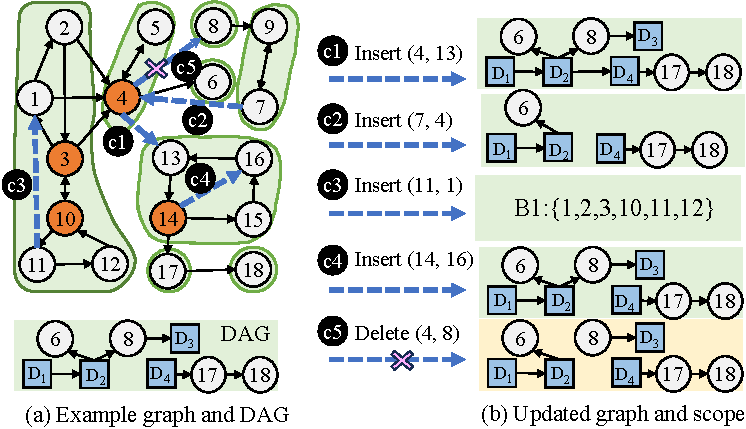
\includegraphics[width=1\linewidth]{figures/update_scope-crop.pdf}
%     \caption{Five scope cases (\circled{c1}--\circled{c5}) for a single edge update on the running example.
%     Cases \circled{c1}--\circled{c4} cover insertions classified by the structural relationship between the
%     two endpoints; \circled{c5} covers deletion, classified by whether the removed edge
%     is a bridge and at which GIR layer.
%     Affected DAG nodes are highlighted in blue; yellow shading indicates a WCC split.}
%     \label{fig:scope-update}
% \end{figure}

% We focus on \textit{single edge update} (insertion/deletion), as node insertions without edges
% do not affect connectivity and node deletions reduce to bulk edge deletions.
% The central challenge is determining which GIR layers are affected by each operation.
% Because GIR stores component labels, SCC membership, DAG ranks, and articulation-point
% metadata for every vertex, this classification requires no graph traversal.
% As illustrated in Figure~\ref{fig:scope-update}, every edge update falls into one of five cases:
% \circled{c1}~$s$ and $t$ reside in \emph{different WCCs} (insertion);
% \circled{c2}~$s$ and $t$ reside in the \emph{same WCC but different SCCs} (insertion);
% \circled{c3}~$s$ and $t$ reside in the \emph{same SCC but different BiCCs} (insertion);
% \circled{c4}~$s$ and $t$ reside in the \emph{same BiCC} (insertion);
% \circled{c5}~edge \emph{deletion}, whose scope depends on bridge status.

% \textbf{Case 1 (Insertion): $s$ and $t$ belong to different WCCs.}
% The inserted edge connects two previously disconnected regions.
% No directed cycle can form across WCC boundaries, and no articulation structure inside
% either component changes.
% The scope is confined to the WCC layer: the two components are merged with an $O(1)$
% label update, and neither the SCC condensation DAGs nor the BC trees are touched.
% \textit{Example.}
% Inserting edge $(4,\,13)$ (\circled{c1}) bridges WCC$_1 = \{1\text{--}12\}$ and
% WCC$_2 = \{13\text{--}18\}$.
% The two condensation DAGs are concatenated into a single one, as shown in
% Figure~\ref{fig:scope-update} (\circled{c1}).

% \begin{figure}[t]
%     \centering
%     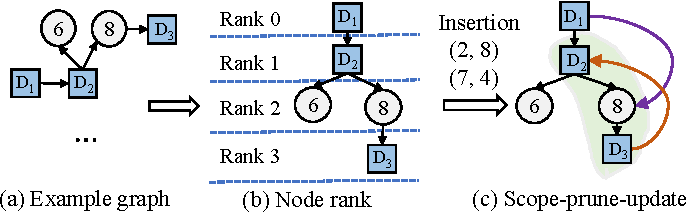
\includegraphics[width=1\linewidth]{figures/scope_update-crop.pdf}
%     \caption{Rank-interval pruning for Case \circled{c2} (inter-SCC insertion).
%     Each SCC is assigned a topological rank in the condensation DAG.
%     When an inserted edge goes against the DAG order from $\mathrm{SCC}(s)$ to
%     $\mathrm{SCC}(t)$, cycle detection is confined to the rank interval
%     $[\mathrm{rank}(\mathrm{SCC}(t)),\,\mathrm{rank}(\mathrm{SCC}(s))]$
%     (shaded region), avoiding a global DAG traversal.}
%     \label{fig:rank-prune}
% \end{figure}

% \textbf{Case 2 (Insertion): $s$ and $t$ are in the same WCC but different SCCs.}
% The inserted edge $s \to t$ introduces a new arc between two SCC supernodes in the
% condensation DAG.
% The critical question is whether this arc creates a directed cycle, which would cause
% two or more SCCs to merge.
% To answer this without traversing the entire DAG, GIR assigns each SCC a \emph{rank}—a
% compact topological index maintained incrementally alongside the condensation DAG.
% If $\mathrm{rank}(\mathrm{SCC}(s)) < \mathrm{rank}(\mathrm{SCC}(t))$, the edge follows
% the existing DAG order and cannot close a cycle; the scope is limited to inserting a
% new DAG arc with no SCC-level structural change.
% If $\mathrm{rank}(\mathrm{SCC}(s)) > \mathrm{rank}(\mathrm{SCC}(t))$, the edge goes
% against the DAG order and may introduce a cycle.
% As illustrated in Figure~\ref{fig:rank-prune}, GIR restricts cycle detection to the
% rank interval $[\mathrm{rank}(\mathrm{SCC}(t)),\,\mathrm{rank}(\mathrm{SCC}(s))]$ in
% the condensation DAG, avoiding a global DAG search.
% If a cycle is confirmed within this interval, all SCCs on the cycle are merged, the
% condensation DAG is updated locally, and the BC trees of the affected SCCs are
% reconstructed.
% \textit{Example.}
% Inserting edge $(5,\,2)$ (\circled{c2}): vertex $5 \in D_2$ and vertex $2 \in D_1$, with
% $\mathrm{rank}(D_2) > \mathrm{rank}(D_1)$ because $D_1 \to D_2$ in the original DAG.
% The edge goes against the DAG direction, so GIR runs cycle detection restricted to the
% interval $[\mathrm{rank}(D_1),\,\mathrm{rank}(D_2)]$ (Figure~\ref{fig:rank-prune}).
% A cycle is confirmed; $D_1$ and $D_2$ are merged, and the BC tree within the new
% combined SCC is updated, as shown in Figure~\ref{fig:scope-update} (\circled{c2}).

% \textbf{Case 3 (Insertion): $s$ and $t$ are in the same SCC but different BiCCs.}
% Both endpoints lie within the same SCC, so no WCC or SCC membership can change.
% The scope is confined to the BiCC layer: specifically, only the two BiCC blocks
% containing $s$ and $t$ are potentially affected.
% The new edge may merge the two blocks into a single larger BiCC, eliminating one or
% more articulation points and updating the BC tree accordingly.
% \textit{Example.}
% Inserting edge $(11,\,1)$ (\circled{c3}): vertex $11$ is in block $b_1 = \{10,\,11,\,12\}$ and
% vertex $1$ is in block $b_2 = \{1,\,2,\,3\}$, both within $D_1$.
% The two blocks merge into $b_1 = \{1,\,2,\,3,\,10,\,11,\,12\}$, as shown in
% Figure~\ref{fig:scope-update} (\circled{c3}).

% \textbf{Case 4 (Insertion): $s$ and $t$ are in the same BiCC.}
% Both endpoints already belong to the same biconnected component.
% Adding an edge within an already 2-edge-connected subgraph cannot create new
% articulation points, split any BiCC block, or alter SCC or WCC structure.
% The update is a structural no-op for all GIR layers; no maintenance is needed.
% \textit{Example.}
% Inserting edge $(14,\,16)$ (\circled{c4}): both vertices lie in the same BiCC block of $D_4$, so
% the GIR remains unchanged (Figure~\ref{fig:scope-update}, \circled{c4}).

% \textbf{Case 5 (Deletion):}
% For deletion of edge $(s,\,t)$, the scope depends on whether the edge is a bridge—
% the sole undirected path between its two endpoints.

% \emph{Case 5a (non-bridge):}
% If parallel edges or alternative undirected paths exist between $s$ and $t$, the
% deletion cannot change WCC, SCC, or higher-level connectivity.
% The scope is confined to the BiCC layer: the removed edge may alter block boundaries
% or articulation structure within the enclosing SCC, but the change does not propagate
% upward.

% \emph{Case 5b (bridge within an SCC):}
% If the edge is the unique undirected path between its endpoints and both endpoints
% share the same SCC, the deletion may split that SCC.
% The scope expands to the SCC layer: GIR checks whether the directed SCC breaks apart
% and, if so, partitions the affected SCC, rebuilds the relevant fragment of the
% condensation DAG, and reconstructs the BC trees of the resulting components.

% \emph{Case 5c (bridge in the condensation DAG):}
% If the deleted edge is an inter-SCC arc and serves as the only undirected path
% connecting two regions of the WCC, its removal disconnects the WCC entirely.
% The scope spans the WCC layer and the BiCC layer: the WCC splits into two independent
% components, the condensation DAG is partitioned accordingly, and the BC trees on each
% side are updated to reflect the new component boundaries.
% \textit{Example.}
% Deleting bridge $(4,\,8)$ (\circled{c5}): edge $4 \to 8$ is the only undirected path between the
% $\{D_1, D_2\}$ side and the $\{6,\,8,\,D_3\}$ side of the graph.
% Its deletion splits the WCC into two components, as shown in
% Figure~\ref{fig:scope-update} (\circled{c5}), requiring both WCC relabeling and BC tree
% updates on each resulting component.

% Table~\ref{tab:updates} summarizes all five cases.
% Only updates that are not structural no-ops proceed to the subsequent Prune and
% Update stages.

% \begin{table}[t]
% \centering
% \small
% \setlength{\tabcolsep}{4pt}
% \renewcommand{\arraystretch}{1.1}
% \caption{Scope rules for single edge update, organized by the five cases.}
% \begin{tabular}{c l l l}
% \toprule
% \textbf{Case} & \textbf{Endpoint relation} & \textbf{Op} & \textbf{Layers affected} \\
% \midrule
% 1 & Different WCCs          & Insert & WCC only\\
% 2 & Same WCC, different SCCs & Insert & SCC + BiCC\\
% 3 & Same SCC, different BiCCs & Insert & BiCC only\\
% 4 & Same BiCC               & Insert & BiCC only\\
% \midrule
% 5a & Non-bridge             & Delete & BiCC only \\
% 5b & Bridge within SCC      & Delete & SCC + BiCC \\
% 5c & Bridge in DAG          & Delete & WCC + BiCC \\
% \bottomrule
% \end{tabular}
% \label{tab:updates}
% \end{table}

% %In GIR, we maintain three layers of structure: WCCs, the SCC condensation DAG, and a per-SCC BC tree.
% %Upon each update, we first apply the gating conditions summarized in Table~\ref{tab:updates} to determine whether the update can affect a given layer.
% %Only the affected layer(s) enter the subsequent prune and update phases; all other cases are treated as no-ops.

% %\YJ{Consider adding examples (in figure) to explain the specific cases.}

% % \subsection{Scope-Prune-Update for Single Edge Updates}

\begin{figure}
    \centering

    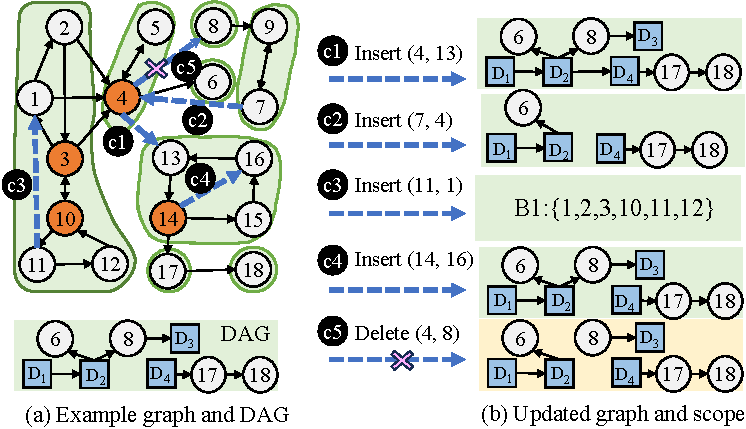
\includegraphics[width=1\linewidth]{figures/update_scope-crop.pdf}
    \caption{Five scope cases (\circled{c1}--\circled{c5}) for a single edge update on the running example.
    Cases \circled{c1}--\circled{c4} cover insertions classified by the structural relationship between the two endpoints; \circled{c5} covers deletion, classified by whether the removed edge is a bridge and at which GIR layer.
    Affected DAG nodes are highlighted in blue; yellow shading indicates a WCC split.}
    \label{fig:scope-update}
\end{figure}

We focus on \textit{single edge update} (insertion/deletion), as node insertions without edges do not affect connectivity and node deletions reduce to bulk edge deletions.
SPU processes each edge update in three steps: \textit{Scope} (classify the update and identify affected layers), \textit{Prune} (restrict the computation to the smallest affected region), and \textit{Update} (perform localized structural repair).

The central challenge is determining which GIR layers are affected by each operation.
Because GIR stores component labels, SCC membership, DAG ranks, and articulation-point metadata for every vertex, this classification requires no graph traversal.
As illustrated in Figure~\ref{fig:scope-update}, every edge update falls into one of five cases:
\circled{c1}~$s$ and $t$ reside in \emph{different WCCs} (insertion);
\circled{c2}~$s$ and $t$ reside in the \emph{same WCC but different SCCs} (insertion);
\circled{c3}~$s$ and $t$ reside in the \emph{same SCC but different BiCCs} (insertion);
\circled{c4}~$s$ and $t$ reside in the \emph{same BiCC} (insertion);
\circled{c5}~edge \emph{deletion}, whose scope depends on bridge status.

We now walk through each case.
For every case, we describe the scope decision (which layers are affected), the pruned region (what subgraph is examined), and the update action (how GIR is repaired).

\textbf{Case 1 (Insertion): $s$ and $t$ belong to different WCCs.}
The inserted edge connects two previously disconnected regions.
No directed cycle can form across WCC boundaries.
No articulation structure inside either component changes.

\textit{Scope.} Confined to the WCC layer only.

\textit{Prune and Update.} The two components are merged with an $O(1)$ label update.
Neither the SCC condensation DAGs nor the BC trees are touched.

\textit{Example.}
Inserting edge $(4,\,13)$ (\circled{c1}) bridges $\text{WCC}_1 = \{1\text{--}12\}$ and $\text{WCC}_2 = \{13\text{--}18\}$.
The two condensation DAGs are concatenated into a single one, as shown in Figure~\ref{fig:scope-update} (\circled{c1}).

\begin{figure}[t]
    \centering

    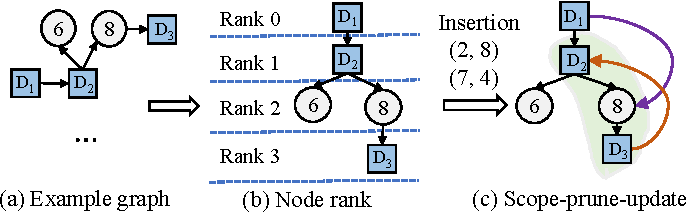
\includegraphics[width=1\linewidth]{figures/scope_update-crop.pdf}
    \caption{Rank-interval pruning for Case \circled{c2} (inter-SCC insertion). Each SCC is assigned a topological rank in the condensation DAG. When an inserted edge goes against the DAG order from $\mathrm{SCC}(s)$ to $\mathrm{SCC}(t)$, cycle detection is confined to the rank interval $[\mathrm{rank}(\mathrm{SCC}(t)),\,\mathrm{rank}(\mathrm{SCC}(s))]$ (shaded region), avoiding a global DAG traversal.}
    \label{fig:rank-prune}
\end{figure}

\textbf{Case 2 (Insertion): $s$ and $t$ are in the same WCC but different SCCs.}
The inserted edge $s \to t$ introduces a new arc between two SCC supernodes in the condensation DAG.
The critical question is whether this arc creates a directed cycle, which would cause two or more SCCs to merge.

\textit{Scope.} To answer this without traversing the entire DAG, GIR assigns each SCC a \emph{rank}, a compact topological index maintained incrementally alongside the condensation DAG.
If $\mathrm{rank}(\mathrm{SCC}(s)) < \mathrm{rank}(\mathrm{SCC}(t))$, the edge follows the existing DAG order and cannot close a cycle; the scope is limited to inserting a new DAG arc with no SCC-level structural change.
If $\mathrm{rank}(\mathrm{SCC}(s)) > \mathrm{rank}(\mathrm{SCC}(t))$, the edge goes against the DAG order and may introduce a cycle.
The scope then expands to the SCC and BiCC layers.

\textit{Prune.} As illustrated in Figure~\ref{fig:rank-prune}, GIR restricts cycle detection to the rank interval $[\mathrm{rank}(\mathrm{SCC}(t)),\,\mathrm{rank}(\mathrm{SCC}(s))]$ in the condensation DAG, avoiding a global DAG search.

\textit{Update.} If a cycle is confirmed within this interval, all SCCs on the cycle are merged, the condensation DAG is updated locally, and the BC trees of the affected SCCs are reconstructed.

\textit{Example.}
Inserting edge $(5,\,2)$ (\circled{c2}): vertex $5 \in D_2$ and vertex $2 \in D_1$, with $\mathrm{rank}(D_2) > \mathrm{rank}(D_1)$ because $D_1 \to D_2$ in the original DAG.
The edge goes against the DAG direction, so GIR runs cycle detection restricted to the interval $[\mathrm{rank}(D_1),\,\mathrm{rank}(D_2)]$ (Figure~\ref{fig:rank-prune}).
A cycle is confirmed; $D_1$ and $D_2$ are merged, and the BC tree within the new combined SCC is updated, as shown in Figure~\ref{fig:scope-update} (\circled{c2}).

\textbf{Case 3 (Insertion): $s$ and $t$ are in the same SCC but different BiCCs.}
Both endpoints lie within the same SCC, so no WCC or SCC membership can change.

\textit{Scope.} Confined to the BiCC layer: specifically, only the two BiCC blocks containing $s$ and $t$ are potentially affected.

\textit{Prune and Update.} The new edge may merge the two blocks into a single larger BiCC, eliminating one or more articulation points and updating the BC tree accordingly.

\textit{Example.}
Inserting edge $(11,\,1)$ (\circled{c3}): vertex $11$ is in block $b_1 = \{10,\,11,\,12\}$ and vertex $1$ is in block $b_2 = \{1,\,2,\,3\}$, both within $D_1$.
The two blocks merge into $b_1 = \{1,\,2,\,3,\,10,\,11,\,12\}$, as shown in Figure~\ref{fig:scope-update} (\circled{c3}).

\textbf{Case 4 (Insertion): $s$ and $t$ are in the same BiCC.}
Both endpoints already belong to the same biconnected component.
Adding an edge within an already 2-edge-connected subgraph cannot create new articulation points, split any BiCC block, or alter SCC or WCC structure.

\textit{Scope.} The update is a structural no-op for all GIR layers; no maintenance is needed.

\textit{Example.}
Inserting edge $(14,\,16)$ (\circled{c4}): both vertices lie in the same BiCC block of $D_4$, so the GIR remains unchanged (Figure~\ref{fig:scope-update}, \circled{c4}).

\textbf{Case 5 (Deletion):}
A \emph{bridge} is an edge whose removal disconnects the subgraph that contains it---formally, an edge $(s,\,t)$ is a bridge if and only if no alternative undirected path connects $s$ and $t$ after its removal.
Bridges are precisely the edges that do \emph{not} belong to any BiCC block of size $\geq 2$; GIR records this status directly, so bridge detection requires no traversal.
The scope of a deletion is determined by where in the GIR hierarchy the bridge sits.

\emph{Case 5a (non-bridge):}
The deleted edge belongs to a BiCC block with at least one alternative path between $s$ and $t$, so no component splits at any level.

\textit{Scope.} Confined to the BiCC layer: the removed edge may change block boundaries or articulation-point status within the enclosing SCC, but the change does not propagate upward.

\textit{Update.} GIR checks whether any articulation points have changed and repairs the BC tree locally.

\emph{Case 5b (bridge within an SCC):}
The deleted edge is a bridge, and both endpoints belong to the same SCC.
Its removal severs the unique undirected path between $s$ and $t$ inside that SCC, which may cause the SCC to split into two or more SCCs.

\textit{Scope.} Expands to the SCC layer: GIR checks whether the directed SCC breaks apart and, if so, partitions it, rebuilds the affected fragment of the condensation DAG, and reconstructs the BC trees of the resulting components.

\emph{Case 5c (bridge in the condensation DAG):}
The deleted edge is an inter-SCC arc and the only undirected path between two regions of the WCC.
Its removal disconnects the WCC entirely.

\textit{Scope.} Spans the WCC and BiCC layers: the WCC splits into two independent components, the condensation DAG is partitioned accordingly, and the BC trees on each side are updated.

\textit{Example.}
Deleting edge $(4,\,8)$ (\circled{c5}): this edge is a bridge because it is the sole undirected path between the $\{D_1, D_2\}$ side and the $\{D_3\}$ side of the WCC (Case~5c).
Its deletion splits the WCC into two components, as shown in Figure~\ref{fig:scope-update} (\circled{c5}), requiring WCC relabeling and BC tree updates on each resulting component.

\begin{table}[t]
    \centering
    \small
    \setlength{\tabcolsep}{4pt}
    \renewcommand{\arraystretch}{1.1}
    \caption{Scope rules for single edge update, organized by the five cases.}
    \begin{tabular}{c l l l}
    \toprule
    \textbf{Case} & \textbf{Endpoint relation} & \textbf{Op} & \textbf{Layers affected} \\
    \midrule
    1 & Different WCCs                & Insert & WCC only\\
    2 & Same WCC, different SCCs & Insert & SCC + BiCC\\
    3 & Same SCC, different BiCCs & Insert & BiCC only\\
    4 & Same BiCC                     & Insert & BiCC only\\
    \midrule
    5a & Non-bridge            & Delete & BiCC only \\
    5b & Bridge within SCC        & Delete & SCC + BiCC \\
    5c & Bridge in DAG            & Delete & WCC + BiCC \\
    \bottomrule
    \end{tabular}
    \label{tab:updates}
\end{table}

Table~\ref{tab:updates} summarizes the scope rules for all five cases.
Case~4 is a complete no-op: no GIR layer requires any maintenance.
For all other cases, the prune step restricts the computation to the smallest affected region, and the update step performs localized structural repair.
This three-step discipline ensures that SPU never performs more work than the structural change requires.


% \subsection{Scope-Prune-Update for Single Update}

% Building on the five-case scope classification above, SPU processes each edge update in three steps.

% \textit{(i) Scope.}
% Classify the update into one of the five cases (Table~\ref{tab:updates}) using stored GIR
% metadata in $O(1)$ time.
% Cases~4 and 5a are structural no-ops and require no further processing.

% \textit{(ii) Prune.}
% Even when a layer is affected, the update typically propagates to only a small region.
% For WCC maintenance, the candidate region is restricted to the component(s) incident to
% the updated edge.
% For SCC maintenance, GIR bounds the search to the rank interval
% $[\mathrm{rank}(\mathrm{SCC}(t)),\,\mathrm{rank}(\mathrm{SCC}(s))]$ in the condensation
% DAG, avoiding a full traversal.
% For BC tree maintenance, repair is confined to the articulation structure local to the
% affected SCC.

% \textit{(iii) Update.}
% Within the pruned region, GIR performs localized structural repair at each affected layer.
% At the WCC layer, components are merged on insertion or split on deletion as needed.
% At the SCC layer, cycle detection within the pruned DAG interval either confirms a merge
% of SCCs or leaves the structure unchanged; for deletions, a reachability check determines
% whether the SCC breaks apart.
% At the BiCC/BC tree layer, block boundaries and articulation points are repaired only
% after the upper layers have stabilized, keeping changes strictly local.

% \subsection{Filter-Merge-Update for Batch Updates}

% %\YJ{Please read the following and think about plotting a figure.}

% FMU extends SPU to batch settings, where multiple updates may overlap, cancel, or jointly trigger structural changes invisible to any single update alone.
% It proceeds in three stages.

% \textit{(i) Filter.}
% The first stage removes redundant, canceling, or structurally irrelevant updates before any maintenance is performed.
% For example, if an edge is inserted and later deleted within the same batch, the two operations cancel out.
% Similarly, some updates can be discarded early because they are guaranteed not to affect the current GIR structure.
% This filtering stage reduces both the number of updates and the amount of downstream recomputation.

% \textit{(ii) Merge.}
% After filtering, the remaining updates are grouped according to the structural regions they may jointly affect.
% Instead of treating every edge independently, GIR merges updates that fall into the same WCC, SCC interval, or local articulation region.
% This merging step amortizes repeated maintenance work across overlapping updates and avoids repeated recomputation on the same region.
% It also provides a natural unit for parallel execution.

% % \YJ{Could add more details.}

% \textit{(iii) Update.}
% Finally, GIR applies the same scope-prune-update logic used for primitive updates, but now at the granularity of merged regions rather than individual edges.
% For example, a set of inserted edges may jointly create a cycle and merge several SCCs, even though none of the edges alone would justify an immediate global update.
% In this case, GIR detects the structural transition over the merged region and repairs the corresponding WCC, SCC, and BC tree structures in a coordinated way.

% Once the batch size is reached, the merged regions are processed concurrently, making FMU a parallel and amortized extension of SPU for high-throughput update streams.


